\subsection{Architektur}
\label{sec:Architektur}

Der Architekturentwurf des vorliegenden Projektes wurde bereits im
\verweis{Architekturgrundlagen} als Ausgangsbasis zur Erläuterung der
technologischen Grundlagen präsentiert. Aufbauend auf diesen Grundlagen wird der
Architekturentwurf im Folgenden genauer betrachtet. Ausgangspunkt der folgenden
Beschriebung ist die Architektur, die in \abbildung{Architektur} dargestellt
ist.

\begin{figure}[htb]
\centering
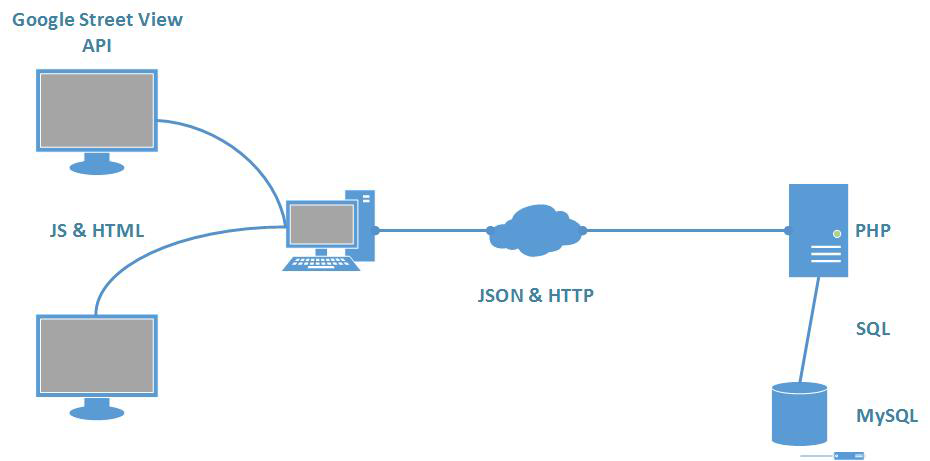
\includegraphics[width=1.0\textwidth]{Architektur.png}
\caption[Architektur der Anwendung]{Architektur der
Anwendung\protect\footnotemark}
\label{fig:Architektur}
\end{figure}
\footnotetext{Quelle: Eigene Darstellung}

Der dargestellte Architekturentwurf zeigt eine klassische
Client-Server-Architektur. Die Architektur lässt sich hierbei in zwei
Subsysteme aufteilen, die über definierte Schnittstellen
miteinander kommunizieren können. Diese Kommunikation erfolgt in Form von
Anfrage und Antwort. Das eine Subsystem fragt dabei einen Dienst an, den das
andere Subsystem anbietet. Das Client-Subsystem ist dabei das Subsystem, welches
einen Dienst anfragt. Das Server-Subsystem bietet hingegen einen solchen
Dienst an\footnote{\citet[S.~177]{rautenstrauch2002}}.

Im vorliegenden Projekt stellt das Server-Subsystem vor allem Webdokumente und
Schnittstellen (APIs) für das Client-Subsystem bereit. Zur Realisierung dieser
Schnittstellen wird die Serverskriptsprache PHP und eine MySql-Datenbank
eingesetzt. Bei der Anfrage eines Webdokuments wird auf dem Serversystem eine
PHP-Routine ausgeführt und als Antwort ein HTML Dokument zurückgeliefert.
Inhalt der PHP-Routine kann dabei eine Anfrage an die Datenbank sein, auf der
aufbauend HTML dynamisch generiert wird.

Bei Anfragen an sogenannte Application Programming Interfaces (APIs) werden
ebenfalls Informationen mit Hilfe von PHP aus der Datenbank gelesen und in
einem definierten Format zurückgeliefert. Im Gegensatz zu Webdokumenten ist
eine solche Schnittstelle (engl: interface) für den Informationsaustausch
zwischen Programmen ausgelegt. Das Ausgabeformat der dargestellten Informationen
ist aus diesem Grund nicht für menschliche Lesbarkeit optimiert.

Die Anfragen an den Server werden durch den Benutzer initiert und die
zurückgelieferten Antworten vom Client interpretiert. Das Clientsystem ist dabei
im vorliegenden Projekt der Internetbrowser eines Benutzers. Dieser löst durch das
Aufrufen von Webseiten anfragen aus, welche vom Server beantwortet werden. Das
hierbei zurückgelieferte HTML wird anschließend durch den Internetbrowser des
Benutzers dargestellt. Eine solche Anfrage ist ein Anwendungsbeispiel für eine
Anfrage nach einem Webdoukment. Über diese Anfragen hinaus werden auf dem Client
Routinen der Programmiersprache Javascript ausgeführt. Durch Javascript können dabei
Benutzerinteraktionen direkt auf dem Client verarbeiten werden. Das steigert die
Performanz, da keine erneuten Anfragen an den Server geschickt werden müssen.
Über diese Technologie ist auch die Google Street View API in die
Anwendung eingebunden. Diese erlaubt es, 360-Grad-Fotos darzustellen und zu
weiteren festgelegten Panoramas zu navigieren.